%\setbeameroption{show notes}
\begin{frame} % Introduction

\begin{center}
\only<1>{
    %
\includegraphics[width=0.5\textwidth]{imgs/profil2.jpg}
    Jáchym Čepický
}

\only<2>{
    
\includegraphics[width=0.3\textwidth]{imgs/Grasslogo_vector_big.png}
    
\includegraphics[width=0.3\textwidth]{imgs/pywps.png}
    \\
    
\includegraphics[width=0.1\textwidth]{imgs/ol.png}
    
\includegraphics[width=0.1\textwidth]{imgs/geopython.png}
    
\includegraphics[width=0.1\textwidth]{imgs/mapserver.png}
    
\includegraphics[width=0.1\textwidth]{imgs/QGis_Logo.png}
    \\
    \dots
}

\only<3>{
    
\includegraphics[width=0.3\textwidth]{imgs/OSGeo_logo_750_317.png}
    ~\url{http://osgeo.org}
    \vfill
    
\includegraphics[width=0.3\textwidth]{imgs/osgeo-cz.png}
    ~\url{http://osgeo.cz}
}

\only<4>{
    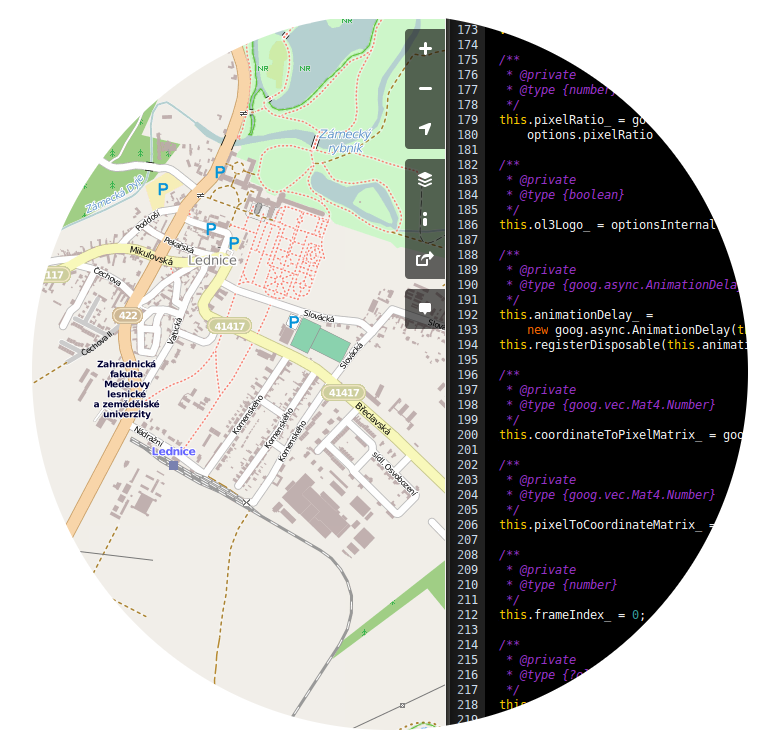
\includegraphics[width=0.7\textwidth]{imgs/map-coding.png}
}
\end{center}

\note<1>{Jmenuji se Jáchym Čepický \\
         Od roku 2002 se pohybují ve světě vývoje Open Source software pro GIS
 }
\note<2>{
    \begin{itemize}
        \item Jsem bývalým členem GRASS Development teamu
        \item původní autor programu PyWPS
        \item přispěvatel do několika dalších projektů, jako jsou například OpenLayers
        \item a uživatel a propagátor otevřeného software pro geooblast.
    \end{itemize}
}
\note<3>{
    Mezi neprogramátorské aktivity patří zejména členství v představuje
    představenstvu Open Source Geospatial Foundation a jsem předseda českého
    sdružení Otevřená geoinfrastruktura.
}

\note<4>{
    Posledních 6 let se zábavám především vývojem webových mapových aplikací pomocí
    různých frameworků a o svoje zkušenosti bych se s vámi dnes rád podělil.
}
\end{frame}

%%%%%%%%%%%%%%%%%%%%%%%%%%%%%%%%%%%%%%%%%%%%%%%%%%%%%%%%%%%%%%%%%%%%%%%%%%%%%%%%%%%%%%
\begin{frame} % Open Source
\begin{center}

\only<1>{
    
\includegraphics[width=0.7\textwidth]{imgs/opensource.png}
}

\only<2-4>{
    \begin{itemize}
        \item<2->Svoboda sdílet
        \item<3->Svoboda měnit
        \item<4->Svoboda sdílet změny
    \end{itemize}
}

\only<5>{
    
\includegraphics[width=0.3\textwidth]{imgs/pivo.jpg}
    ~\alert{$\times$}~
    
\includegraphics[width=0.3\textwidth]{imgs/freedom.jpg}
}


\only<6>{
    \begin{itemize}
        \item\alert{Svoboda} sdílet
        \item\alert{Svoboda} měnit
        \item\alert{Svoboda} sdílet změny
    \end{itemize}
}

\note<1>{
    Nejdříve si musíme vymezit pojmy a tím prvním v záhlaví této přednášky je termín
    Open Source.\\ ~ \\

    Omlouvám se, pokud máte pocit, že toto téma pro vás není nic
    nového. Zkušenost posledních let ale i měsíců mě však nutí vymezit tuto
    problematiku alespoň okrajově. \\ ~ \\

    Pod tímto - tedy open source, otevřený softwate
    - pojmem zahrnuji skupinu software, který je uvolněn pod určitou licencí, která
    přiznává uživateli tohoto software určitá práva, někdo by řekl, že svobody nebo
    podmínky:
}
\note<2-4>{
    \begin{itemize}
        \item Svobodu sdílet - dále distribuovat program dalším uživatelům\mynext
        \item Svobodu měnit program\mynext
        \item Svobodu sdílet tyto změny s dalšími uživateli
    \end{itemize}
}

\note<5-6>{
    Díky těmto právům a svobodám se někdy hovoří o Svobodném software nebo Free
    Software (psáno s velkým F), v angličtině je někdy význam slova Free mylně
    chápán ve smyslu ceny - free as a beer - zadarmo jako pivo.  Ale znamená to
    skutečně svobodný od slova svoboda (nebo free as freedom) a jsou tím myšlena ona
    tři práva\mynext
    \\ ~ \\
    sdílet, měnit a sdílet změny.
}
\end{center}
\end{frame}

%%%%%%%%%%%%%%%%%%%%%%%%%%%%%%%%%%%%%%%%%%%%%%%%%%%%%%%%%%%%%%%%%%%%%%%%%%%%%%%%%%%%%%
\begin{frame} % Open Source
\begin{center}
\only<1>{
    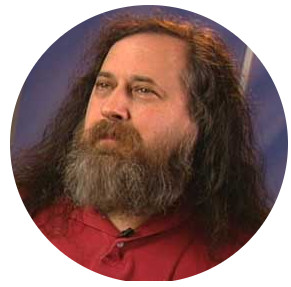
\includegraphics[width=0.5\textwidth]{imgs/rms.jpg}
    \hfill
    
\includegraphics[width=0.5\textwidth]{imgs/gnu.jpg}
    \\
    Richard Matthew Stallman, 1983 -- Operační systém GNU
}

\only<2>{
    \textbf{Věda}
    \begin{itemize}
        \item výzkum
        \item publikace
        \item ověření výsledků
    \end{itemize}
}

\only<3>{
    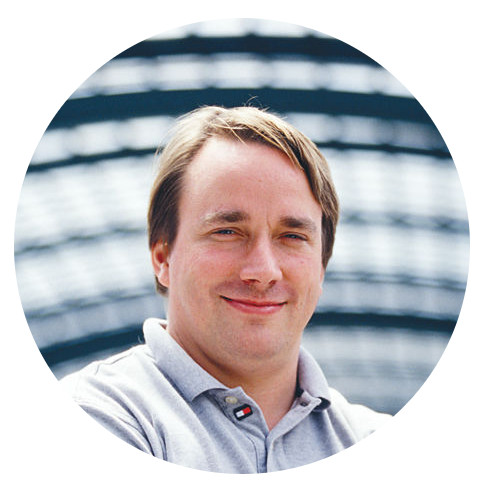
\includegraphics[width=0.5\textwidth]{imgs/linus.jpg}
    \hfill
    
\includegraphics[width=0.35\textwidth]{imgs/Tux.png}
    \\
    Linus Torvalds, 1991 -- Jádro systému Linux
}

\only<4>{
    \begin{quote}
        Only wimps use tape backup: real men just upload their important stuff
        on ftp, and let the rest of the world mirror it ;)
    \end{quote}
    \begin{flushright}
    -- Linus Torvalds, 1996
    \end{flushright}
}

\only<5>{
    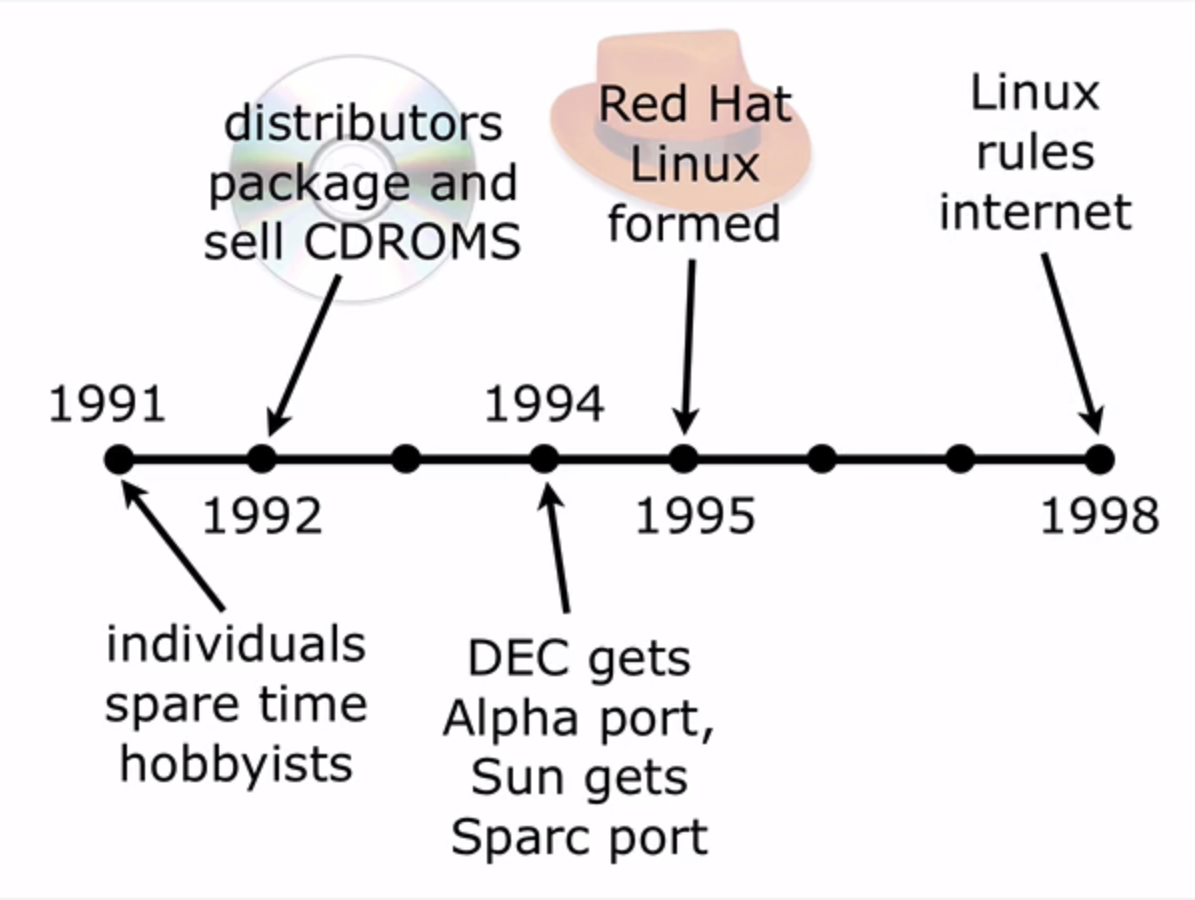
\includegraphics[width=0.75\textwidth]{imgs/linux-history.png}
    \begin{flushright}
        \emph{zdroj: P. Ramsey, Open Source and the Spatial Web,
        \url{http://vimeo.com/92522557}}
    \end{flushright}
}

\only<6>{
    
\includegraphics[width=0.35\textwidth]{imgs/community.jpg}
}


\only<7>{
    \begin{itemize}
        \item\alert{Svoboda} sdílet
        \item\alert{Svoboda} měnit
        \item\alert{Svoboda} sdílet změny
    \end{itemize}
}

\note<1>{
    Možná máte pocit, že Svobodný software je něco nového. Z pohledu IT světa byl
    ale tento koncept pojmenován v 80. letech Richardem Stallmanem, který založil
    nadaci Free Software Foundation a začal spolu s ostaními pracovat na svobodném
    operačním systému. Vzali to opravdu z gruntu  - nejdříve naprogramovali textový
    editor pro psaní zdrojového kódu a pokračovali kompilátorem zdrojového kódu.
}

\note<2>{
    Přesto ale, koncept sdílení je základ naší vědeckého pokroku naší západní
    cilivizace. Pokud oběvíte něco nového o čem se domníváte, že stojí za to
    zveřejnit, tak publikujete výsledky svého výzkumu v časopise. Očekává se, že váš
    popis problému a vašeho řešení bude takový, že někdo jiný jej může zopakovat,
    aby vaše závěry potvrdil nebo vyvrátil. Může eventuálně váš pokus změnit a
    publikovat opět své výsledky s pozměněným postupem.
}

\note<3>{
    Richard Stallman spolu se svými kolegy naprogramovali kompletní operační systém,
    jediné co jim do dnes chybí, je jádro systému, což je část, která je odpovědná
    za komunikaci s hardwarem, tedy "železem". V roce 1991 ale jistý finský student
    začal pracovat na takovém jádru a zveřejnil je pod svobodnou licencí General
    Public License - GPL.
}

\note<4>{Zcela v souladu se svým výrokem "jenom srabi zálohují,
    opravdoví muži nahrají svou práci na FTP a nechají ostatní, aby si stáhli kopii"
    toto jádro zpřístupnil ostatním pod názvem Linux.
}

\note<5>{
    Linux byl použit pro operační systém GNU a ten se stal tak úspěšným, že po
    sedmi letech se stal nejčastěji používaným operačním systémem na
    internetových serverech.  Trvalo 7 let od prototypu až po dobu, kdy
    GNU/Linux byl akceptován podnikovou sférou. Stalo se tak bez marketingového
    oddělení, bez liceční politiky, bez faktického vlastnictví, přímých prodejů
    nebo jakékoliv kontroly.
}
\note<6->{
    Celé to ale není práce jednoho nebo dvou lidí. Je to spolupráce obrovské
    komunity vývojářů, kteří spolu navzájem sdílejí práci. Proč by ale někdo sdílel
    svou práci s ostatními?\mynext \\
    ~ \\
    Protože Linux je Open Source a tak jakákoliv práce
    někoho jiného je okamžitě přístupná všem ostatním.
}
\end{center}
\end{frame}

%%%%%%%%%%%%%%%%%%%%%%%%%%%%%%%%%%%%%%%%%%%%%%%%%%%%%%%%%%%%%%%%%%%%%%%%%%%%%%%%%%%%%%
\begin{frame} % Intelectual commons
\begin{center}
Open Source vytváří\\
\textbf{Intelektuální spoluvlastnictví}

\note{
    Open Source vytváří intelektuální spoluvlastnictví, které nikdy nemůže být
    eliminováno. Lidé se chtějí na tomto bohatství podílet způsobem, jakým by se asi
    nikdy nepodílely na soukrém vlastnictví. Lidé celkem ochotně zvláště teď na jaře
    uklízejí odpadky v lesích a na cestách, ale můj trávník mi nikdo neposeká.
    \\
    ~
    \\
    Ale Open Source není izolovaným příkladem tohoto společenského hnutí. Díky
    internetu vznikla celá řada dalších společných intelektuálních bohatství.
}
\end{center}
\end{frame}

%%%%%%%%%%%%%%%%%%%%%%%%%%%%%%%%%%%%%%%%%%%%%%%%%%%%%%%%%%%%%%%%%%%%%%%%%%%%%%%%%%%%%%
\begin{frame} % Intelectual commons
\begin{center}

\only<1>{
    
\includegraphics[width=0.5\textwidth]{imgs/wikipedia.jpg}
}

\only<2>{
    
\includegraphics[width=0.2\textwidth]{imgs/cc.png}\\
    Creative Commons
    \begin{itemize}
        \item sdílet
        \item měnit
        \item sdílet změnu
    \end{itemize}
}


\note<1>{
    Takovým příkladem může být úspěšná encyklopdie Wikipedia, která zatlačila do
    pozadí encyklopedii Britanica. Britanica v podstatě skončila, protože byla
    převálcována ne National Geographic nebo jiným úspěšným mediální domem. Ale
    komunitou soustředěnou okolo jednoho projektu, sdílející společné vědomosti.
    Není to tak, že by se to stalo ze dne na den. Britanica samozřejmě tento proces
    sledovala po několik let, ale nedokázala jej zastavit. Nemohli spustit
    wiki.britanica.com, protože nikdo by jim nepřispíval. Nikdo nechce pracovat
    zadarmo pro někoho jiného. Lidé raději pracují na wikipedii, ale proč?
}
\note<2>{
    Protože
    díky licenci, kterou Wikipedia používá - Creative Commons, což je vlastně open
    source licence - můžete sdílet, měnit a sdílet změněnou informaci s ostaními a
    ostatní s vámi. Tato prezentace je mimochodem dostupná pod licencí Creative
    Commons na githubu.
}
\end{center}
\end{frame}

%%%%%%%%%%%%%%%%%%%%%%%%%%%%%%%%%%%%%%%%%%%%%%%%%%%%%%%%%%%%%%%%%%%%%%%%%%%%%%%%%%%%%%
\begin{frame} % OSM
\begin{center}
\only<1>{
    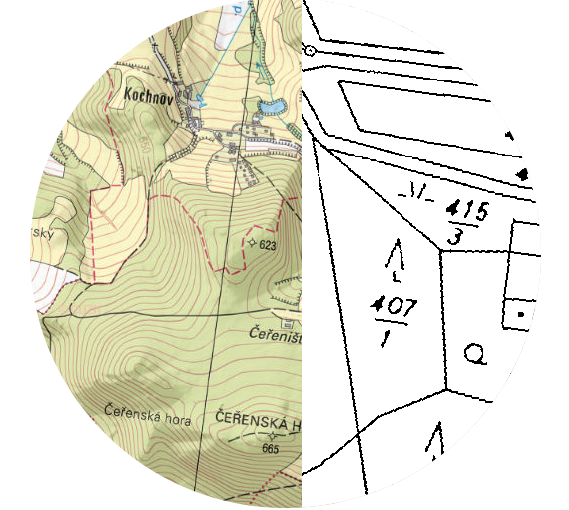
\includegraphics[width=0.5\textwidth]{imgs/smd.png}
}
\only<2>{
    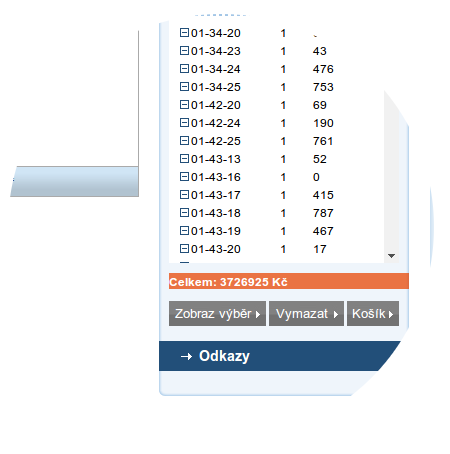
\includegraphics[width=0.5\textwidth]{imgs/zabaged-cena-circle.png}\\
    Celkem: 3~726~925 Kč\\
    \url{http://geoportal.cuzk.cz/(S(pi4gmefgc1dw3s55gomgoo45))/Default.aspx?mode=eShop\&head_tab=sekce-01-gp\&menu=13}
}
\only<3>{
    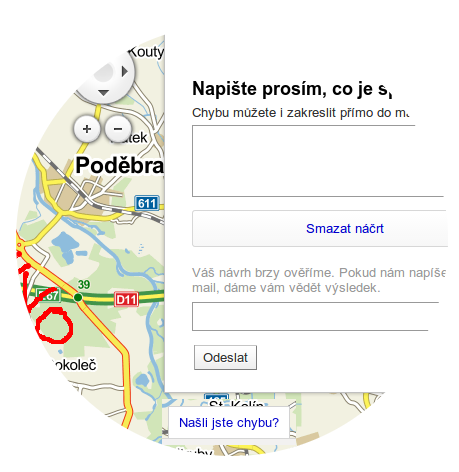
\includegraphics[width=0.5\textwidth]{imgs/seznam.png}
}
\note<1>{
    Tím se dostáváme od obecného ke konkrétnímu -- k geoinformatice. Asi víte že
    většina geodat v České republice je vytvářena a spravována českým úřadem
    zeměměřičským a katastrálním. Autorský zákon obsahuje výjimku, na základě
    které úřední díla jsou automaticky přístupná všem. Pouze s výjimkou státního
    mapového díla, kde pro volné použít je dostulná pouze katastrální mapa a to
    jen proto, že se zde nepřipouští žádná tvůrčí autorská invence. Ostatní
    části státního mapového díla jsou šířeny za poměrně tvrdých licenčních
    podmínek.
}

\note<2>{
    Pokud potřebujete například  polohopisnou mapu Základní báze geografických
    dat, tak si ji musíte koupit, protože tyto data mají výjimku z výjimky
    autorského zákona. Autorský zákon v České republice explicitně říká, že
    veškerá úřední díla jím nejsou chráněna. Co je ale základní mapa jiného, než
    úřední dílo? Vzniká za státní peníze, spravuje ji státní instituce ... proč
    ta data nemůžeme volně používat?  Ta data si můžete koupit. Česká republika
    jako celek vás vyjde na bratru 4 miliony korun, ale myslím, že byste dostali
    množstevní slevu 10\%.  Ortofoto by vás vyšlo na Celkem:
    2~366~501~Kč
}
\note<3>{
    Samozřejmě můžete používat mapy komerčních firem, ty jsou levnější (i když data
    vám nikdo nenabídne, maxilně obrázky v podobě dlaždic) a dokonce můžete tato
    data pomocí nástrojů pomáhat vylepšit a funguje to, sám jsem si to zkusil.
    Nevím, jestli  jste to někdy udělali, ale nemáte pocit, že ten vztah je trochu
    nevyvážený? Vy opravítě pokladová data a vaši práci, vaše intelektuální
    vlastnictví, použije nějaká firma pro vylepšení své roční bilance?
}
\end{center}
\end{frame}

%%%%%%%%%%%%%%%%%%%%%%%%%%%%%%%%%%%%%%%%%%%%%%%%%%%%%%%%%%%%%%%%%%%%%%%%%%%%%%%%%%%%%%
\begin{frame} % OSM
\begin{center}
\only<1>{
    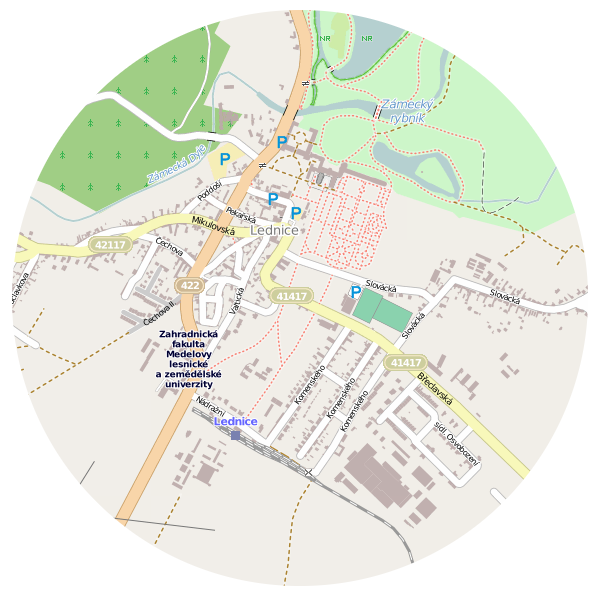
\includegraphics[width=0.5\textwidth]{imgs/osm.png}
}

\only<2>{
    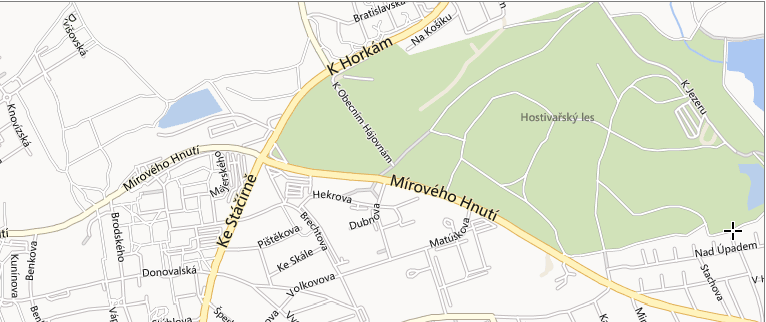
\includegraphics[width=0.8\textwidth]{imgs/osm-bing.png}\\
    Bing
}
\only<3>{
    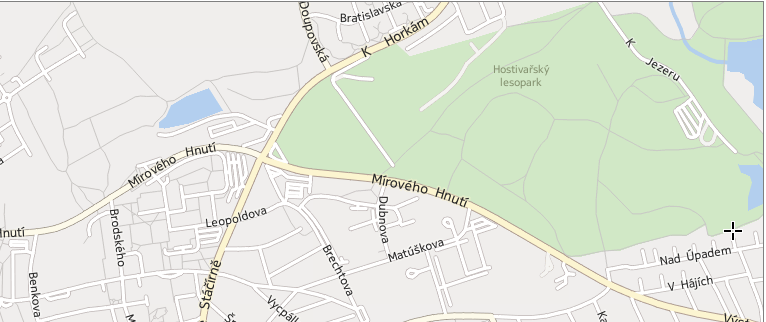
\includegraphics[width=0.8\textwidth]{imgs/osm-here.png}\\
    Here
}
\only<4>{
    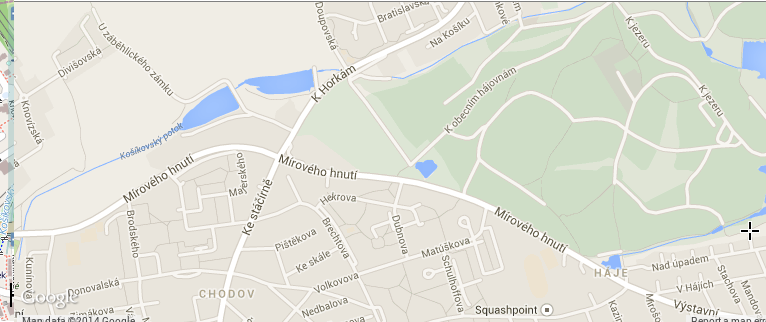
\includegraphics[width=0.8\textwidth]{imgs/osm-google.png}\\
    Google
}
\only<5>{
    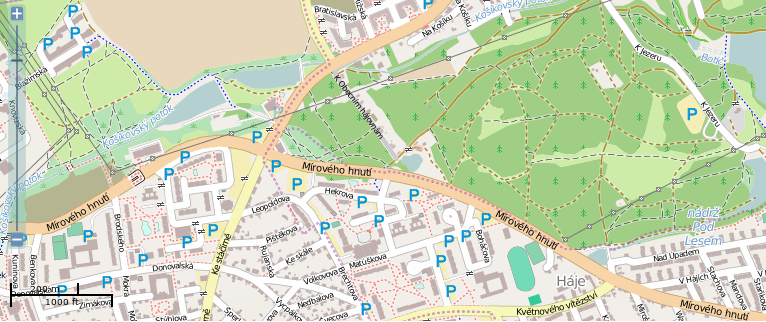
\includegraphics[width=0.8\textwidth]{imgs/osm-osm.png}\\
    OSM
}
\only<2-5>{
    \url{http://tools.geofabrik.de/mc}
}

\only<6>{
    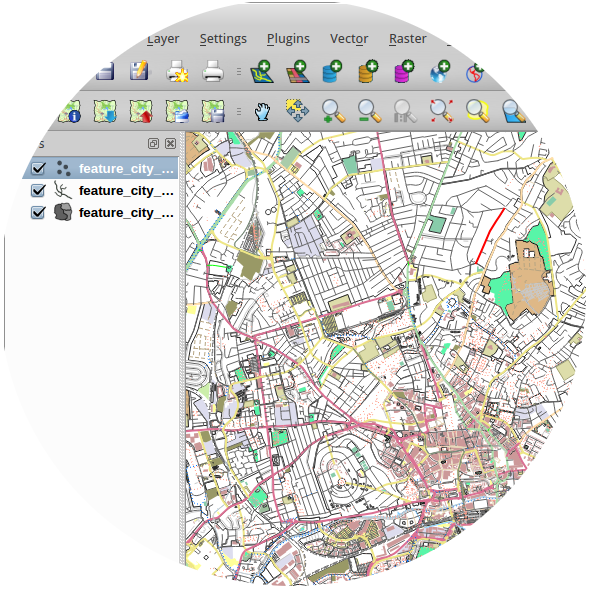
\includegraphics[width=0.5\textwidth]{imgs/osm-vectors.png}
}

\note<1>{
    V roce 2007 ale začal malý universitní projekt jménem OpenStreetMap, který měl
    za cíl vytvořit společné intelektuální vlastnictví geodat. Tento projekt je
    velice úspěšný, protože zaplnil poptávku, hlad po dobrých geodatech nebo po
    geodatech, která jsou "dostatečně dobrá". Jejich licence umožňuje data sdílet,
    měnit a opět sdílet.
}
\note<2-5>{
    Na internetu můžete najít celou řadu konkrétních srovnání
    mezi různými službami, jako je Bing maps, \mynext \\
    ~ \\
    Nokia mapy \mynext nebo Google  a
    OpenStreetMap, kdy OpenStreetMap \mynext \\
    ~ \\
    vyjde jako zdroj s nejlepším pokrytím. V České
    republice někdy vychází lépe OpenStreetMap, někdy komerční mapy. Co je ale
    podstatné: Existuje datový zdroj, otevřený datový zdroj, který nabízí data pro
    vaše použití.
}

\note<6>{
    Ne jen předgenerované dlaždice - obrázky, ale původní data se
    vším, co se do dlaždic nevešlo. A ta data jsou pro řadu aplikací dostatečně
    kvalitní. Projekt, který při pohledu z venčí dělá pár bláznů s GPSkami je
    nebojím se to říci veleúspěšný a zdatně konkuruje komerčním projektům, za
    kterými stojí finančí kapitál nebo státní peníze. Ten projekt vzniknul z
    potřeby, z nedostatku legálních dat. Kdyby existovala dostupná otevřená geodata,
    pravděpodobně by nikdy nebyl potřeba. Pokud potřebujete data přes celou
    republiku, neřku-li Evropu, víte kam sáhnout.  Nastávají z mého pohledu absurdní
    situace, kdy veřejné instituce, než aby řešili licence a nákup a poskytování dat
    s pověřenou osobou (jako příklad můžeme vzít právě český zěměměřicský úřad),
    raději použijí OpenStreetMap pro své interní potřeby. 
}
\end{center}
\end{frame}

%%%%%%%%%%%%%%%%%%%%%%%%%%%%%%%%%%%%%%%%%%%%%%%%%%%%%%%%%%%%%%%%%%%%%%%%%%%%%%%%%%%%%%
\begin{frame} % open source closure
\begin{center}
\only<1>{
    
\includegraphics[width=0.4\textwidth]{imgs/wikipedia.jpg}
    
\includegraphics[width=0.3\textwidth]{imgs/osm-logo.png}\\
    
\includegraphics[width=0.3\textwidth]{imgs/opensource.png}
}
\only<2>{
    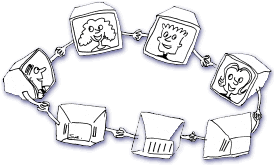
\includegraphics[width=0.4\textwidth]{imgs/internet-community.png}
}

\only<3>{
    Sdílení a spolupráce není nic neobvyklého
}

\only<4>{
    Sdílení a spolupráce \textbf{je normální}
}

\only<5>{
    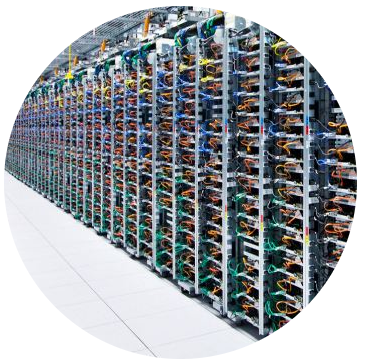
\includegraphics[width=0.4\textwidth]{imgs/google-servers.png}
}


\note<1>{
    Abych tuto část nějak uzavřel: Open Source software je jenom jedna část tohoto
    způsobu vytváření společné znalostní báze. Ale stejným způsobem pracuje
    Wikipedia nebo OpenStreetMap. Komunity spojené internetem vytvářejí hodnoty, pro
    jejichž vytvoření byly dříve potřeba velké instituce.
}

\note<2>{
    Může to znít jako pohádka. Ale ve skutečnosti je to kombinace společných potřeb a
    zájmů, pravidel pro sdílení, která nikoho nestaví do podřízenecké role, a
    moderních komunikačních technologií, které umožňují spolupráci lidí, kteří se
    nikdy neviděli.
}

\note<3-4>{
    Open Source software a otevřený způsob spolupráce není nějaké náboženství,
    nneí to abnormalita.\mynext\\
    ~ \\
    Je to prostě normální. Lidé spolu sdíleli svoje znalosti v minulosti a dělají tak i v
    současnosti. Otevřenost je norma. Open Source software je všude kolem nás.
}
\note<5>{
    Google by nebyl čím je bez tisíců linuxových serverů, na kterých běží.
 Facebook by neexistoval ze stejného důvodu. \\
 ~\\
    Android používá linuxové jádro. Tyto úspěšné
    firmy nejen že používají Open Source (v případě Facebooku např. MySQL, PHP,
    samozřejmě také Linux), ale sami jej aktivně vytváří -- Google mimo jiné
    prohlížeč Chromium, javascriptovou knihovnu Closure, Facebook úspěšný
    šablonovací systém React nebo nosql databázi Cassandra. Většina vašich routrů
    doma používá Open Source. 
}
\end{center}
\end{frame}

%%%%%%%%%%%%%%%%%%%%%%%%%%%%%%%%%%%%%%%%%%%%%%%%%%%%%%%%%%%%%%%%%%%%%%%%%%%%%%%%%%%%%%
\begin{frame} % open source geo
\begin{center}
Open Source Geo-
\begin{itemize}
    \item<2-> Používám, co znám
    \item<3-> Změna bolí
    \item<4-> Kde začít?
\end{itemize}

\note<1>{
    Takže jak je to v našem geosvětě s open source? No, očekával bych asi větší
    podporu pro Open Source technologie v české geo-komunitě, než jakou vidím. Ale
    proč to tak je?
}

\note<2>{
    Především - lidé používají co znají, co je "normální". Normální je, co znáte ze
    školy, s čím jste vyrostli, co vás provází vaším profesním životem.
}

\note<3>{
    Zadruhé je to množství znalostí, které potřebujete na začátku, než můžete
    software začít používat. Změna vždycky bolí. Projekty se snaží zploštit tak
    zvanou křivku učení, ale pro někoho je prostě stále příliš exponciální.
}

\note<4>{
    A nakonec: Open Source nemá marketingové oddělení. Není tu nikdo kdo by vám
    řekl, že potřebujete tu a tu funkci. Lidé mají tendenci zkracovat a říkat, že
    potřebují ten a ten konkrétní produkt, místo aby se nejdříve zamysleli nad
    celkovou architekturou a teprve podle té mohou udělat dobré rozhodnutí o tom,
    jaký proudukt tyto potřeby splňuje.
}
\end{center}
\end{frame}

%%%%%%%%%%%%%%%%%%%%%%%%%%%%%%%%%%%%%%%%%%%%%%%%%%%%%%%%%%%%%%%%%%%%%%%%%%%%%%%%%%%%%%
\begin{frame} % open source geo
\begin{center}

\begin{itemize}
    \item<2->Databázový server \only<6->{ -- PostGIS}
    \item<3->Mapový server \only<7->{ -- MapServer}
    \item<4->Dlaždicová cache \only<8->{ -- MapCache}
    \item<5->\only<5-8>{Webová aplikace}\only<9->{\alert{Webová aplikace}}
\end{itemize}

\note<1>{
    Abych to vzal od začátku: každá webová aplikace bez ohledu jestli open
    source nebo postavená z proprietárních komponent má tři nebo čtyři základní komponenty:
}
\note<2>{
    Někde na serveru jsou surová data v nějaké databázi.
}
\note<3> {
    Z těchto dat jsou generovány kartografické a datové výstupy pomocí nějakého
    mapového serveru.
}
\note<4>{
    Pokud chcete věci zrychlit, použite často caschovací mezivrstvu, která ukládá
    předgenerované dlaždice a může tak rychleji s menší režijí vybavit  požadavky
    klienta.
}
\note<5>{
    A konečně na klinetské straně je nějaká webová stránka, která zobrazuje tyto
    obrázky. Všechny moderní open source nebo komerční systémy používají pro
    účely zobrazení program napsaný v programovacím jazyk JavaScript.  U
    starších systémů se můžete setkat s Flashem nebo SilverLightem. Mapa mluví
    buď přímo se serverem a dostává čerstvě vyrenderovaná nebo přímo surová
    data, nebo s dlaždicovou cashí a dostává předgenerované statické dlaždice a
    uspořádá je do mapového pohledu.
}

\note<6-8>{
    Asi mi věříte, že bychom mohli jednotlivé části tohoto stacku hodiny
    rozebírat a zvažovat aspekty různých softwarových balíků, ať už jsou open
    source nebo proprietární. Asi vás nepřekvapí, že na serveru bych já asi
    zvolil databázi PostgreSQL s nadstavbou PostGIS, \mynext\\
    ~\\
    mapový server bych nasadil MapServer nebo GeoServer \mynext\\
    ~\\
    na cache bych nasadil např. MapCash.
}

\note<9>{
    Tato přednáška by se ale měla týkat především té klientské webové části -
    frontendu, přes který komunikují přímo uživatelé. Je důležité zmínit, že ať
    už použijete jakýkoukoliv technologii na straně serveru v některé z jeho
    částí, držte se standardů OGC a zvažujte vzájemnou kompatibilitu a
    interoperabilitu. Tím si zajistíte, že budete v budoucnu schopni
    nevyhovující technologii nahradit jinou, ať už to bude z technologických,
    licenčních nebo výkonnostních důvodů.
}
\end{center}
\end{frame}
%%%%%%%%%%%%%%%%%%%%%%%%%%%%%%%%%%%%%%%%%%%%%%%%%%%%%%%%%%%%%%%%%%%%%%%%%%%%%%%%%%%%%%
\begin{frame} % 
\begin{center}
Bez programování to nejde

\note{
    Chcete dělat mapy na webu? Bez programování se neobejdete, pokud vám tedy
    nestačí jednoduché klikání v některém z vyšších frameworků a nastavení
    kartografie na straně serveru. Potom se ale obávám, že se nedostanete dále
    než naklikání pravidel na desktopu a vypublikování dat formou rastrovaných
    vektorů.\\
    ~\\
    Jděte a programujte. Vyberte si nějaký jazyk typu Python nebo JavaScript a
    začněte tvořit.
    
}
\end{center}
\end{frame} % open source javascript mapping frameworks
    

%%%%%%%%%%%%%%%%%%%%%%%%%%%%%%%%%%%%%%%%%%%%%%%%%%%%%%%%%%%%%%%%%%%%%%%%%%%%%%%%%%%%%%
\begin{frame} % open source javascript mapping frameworks
\begin{center}

\includegraphics[width=0.2\textwidth]{imgs/ol.png}\hspace{0.1\textwidth}

\includegraphics[width=0.2\textwidth]{imgs/leaflet.png}\hspace{0.1\textwidth}

\includegraphics[width=0.2\textwidth]{imgs/ol3.png}\\

\includegraphics[width=0.2\textwidth]{imgs/d3.png}

\note{
    Pokud se posuneme na stranu klienta a webového prohlížeče, máme na výběr v
    podstatě ze tří hlavních možností: OpenLayers, Leaflet a OpenLayers 3.\\
    ~\\
    Určitým způsobem, z hlediska webové kartografie, do tohoto souboru určitě
    patří i knihovna D3.js
}
\end{center}
\end{frame} % open source javascript mapping frameworks
    

%%%%%%%%%%%%%%%%%%%%%%%%%%%%%%%%%%%%%%%%%%%%%%%%%%%%%%%%%%%%%%%%%%%%%%%%%%%%%%%%%%%%%
\begin{frame} % openlayers 2
\begin{center}
\begin{flushright}
    
\includegraphics[width=0.08\textwidth]{imgs/ol.png}
\end{flushright}
\only<1>{
    \begin{itemize}
        \item MetaCarta 2005
        \item Google Maps  API
        \item SVG, VML
        \item 2.13
        \item OGC OWS (WMS, WFS, WPS, \dots), GML, GeoJSON, GeoRSS, GPX
        \item Google Maps, Bing, ESRI ArcIMS
    \end{itemize}
}

\only<2> {
    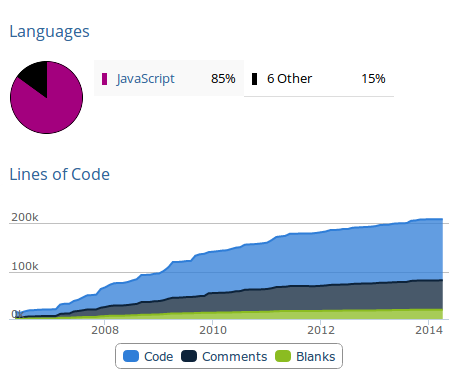
\includegraphics[width=.7\textwidth]{imgs/ol-ohloh-code.png}
    \url{http://www.ohloh.net/p/openlayers/}
}

\only<3> {
    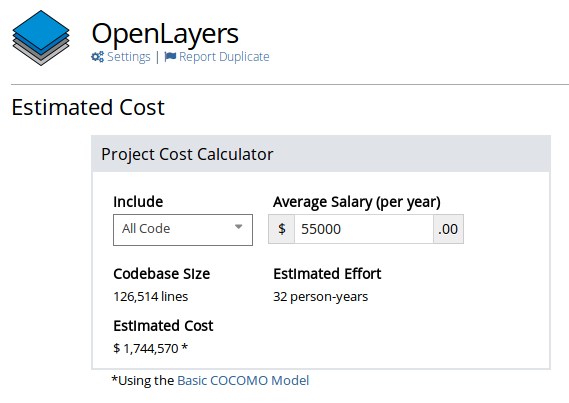
\includegraphics[width=.7\textwidth]{imgs/ol-ohloh-costs.png}
    \url{http://www.ohloh.net/p/openlayers/}
}

\only<4> {
    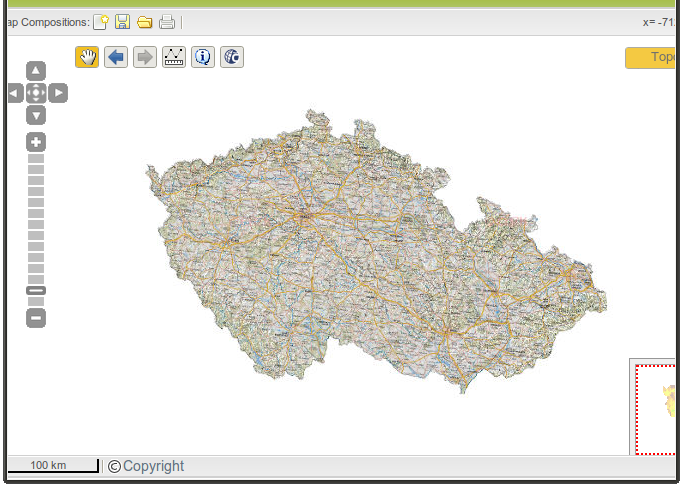
\includegraphics[width=.7\textwidth]{imgs/portal-inspire.png}\\
    \url{http://geoportal.gov.cz}
}

\only<5->{
    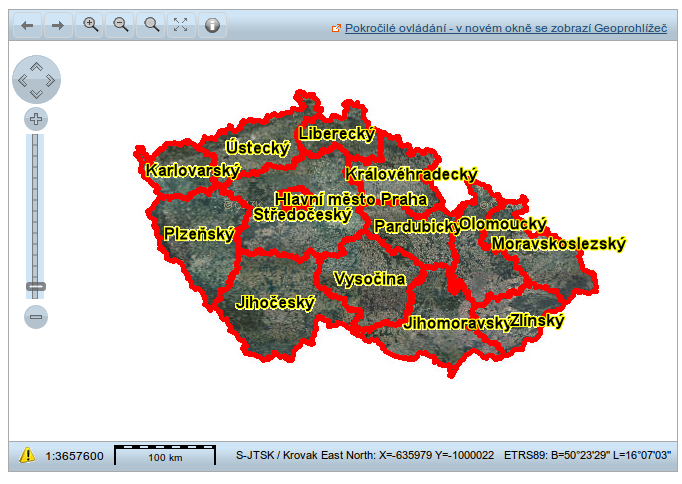
\includegraphics[width=.7\textwidth]{imgs/portal-cuzk.png}\\
    \url{http://geoportal.cuzk.cz}
}

\note<1>{
    OpenLayers je nejstarší a tudíš nejstabilnější projekt z těchto tří zmíněných.
    Začala je vyvíjet firma MetaCarta v roce 2005. První představení Open Sourcové
    veřejnosti proběhlo na konferenci FOSS4G (Free and Open Source Software for
    Geoinformatics) v roce 2006. OpenLayers tenkrát bylo menší senzaci. Musíme si
    uvědomit, že od roku 2005, kdy Google představil svoje mapové rozhraní a v
    podstatě redefinoval způsob, jakým jsme se do té doby dívali na webové mapové
    aplikace, neexistovala použitelná Open Source alternativa ke Google Maps.
    Všichni tedy čekali na něco nebo někoho, kdo se toho chopí a OpenLayers rychle
    získaly na popularitě. Projekt rostl prakticky do minulého roku. Snažil se vždy
    podporovat všechny prohlížeče na trhu. Používal tehdy moderní technologie pro
    vykreslování dat, jako je SVG - Scalable Vector Graphics pro webové prohlížeče,
    a Vector Markup Language Language pro Internet Explorer. Mají podporu pro
    dlaždicované mapy. OpenLayers jsou momentálně ve verzi 2.13 a obsahují podporu
    pro celou řadu rastrových a vektorových formátů. Z rastrových bych uvedl WMS,
    WMTS, prostý obrázek. Z vektorových GML, GeoJSON, GeoRSS, GPX a další. Obsahují
    také podporu pro komernčí API jako je Google Maps, BING. Obsahují také podporu
    prorietárních protkolů, jako ESRI ArcIMS. Lze je využít na práci s dalšími
    komunikačními protokoly, jako je parsrování GetCapabilities pro WMS a WFS,
    kompletní podpora pro OGC Web Processing Service a další a další. 
}
\note<2>{
    Z pohledu vývojářského je to čistě JavaScriptová knihovna, která má něco okolo 4
    MB zdrojového kódu. Je to napsáno velice čistě a standardy pro přijmutí patche -
    (nebo) opravy zdrojového kódu byly nastaveny ve srování s jinými projekty, se
    kterými jsem měl do té doby nějakou zkušenost, velice vysoko. Kromě pevně daného
    coding starndardu je celý zdrojový kód pokryt unit testy. Co to všechno znamená:
    OpenLayers je stabilní, dlouhodobě udržovaný a udržitelný projekt. Podíváte-li
    se na aktivitu OpenLayers např. na serveru Ohloh zjistíte, že OpenLayers mají
    celkem 114 přispěvatelů do zdrojového kódu. Nejvíce aktivních vývojářů bylo v
    roce 2012 - celkem 21.
}
\note<3>{
    Celkové náklady na vývoj jsou odhadovány podle serveru
    Ohloh na \$1.7Mil, při 32 člověko-letech práce a ročních nákladech na vývojáře
    \$55000. Bavíme se o 126 000 řádcích zdrojového kódu. Tím chci říct, že vývoj
    Open Source software není zadarmo. U takto velkého projektu je potřeba zaplatit
    kvalifikované vývojáře a u OpenLayers se to daří. Většina kódu byla de-facto
    zaplacena několika firmami, zejména firmou MetaCarta a Boundless (dříve
    OpenGeo). To jsou firmy, které dlouhodobě investují do vývoje Open Source
    mapových softwarů a jsou skutečně leadry v oboru. Kde se používají?
}
\note<4-5> {
    V České republice je najdete např. na národním Geoportálu INSPIRE nebo na
    portálu ČUZK.\mynext\\
    ~\\
    Ten dělala firma Integraph, kterou si dovolím označit za
    všechno možné - jen ne Open Source - pozitivní firmu. OpenLayers jim ale
    nevadí.
}

\note<6>{
    Po nějaké době OpenLayers jako projekt poněkud zbytněl. Začal obsahovat funkce,
    které jste z 90\% nevyužili. Ví někdo, co je to WPS a použitl to někdo z vás na
    webu? Takže pro většinu z vás je informace, že OpenLayers obsahují podporu pro
    OGC WPS asi nic moc říkající (jakkoliv může být důležitá pro mě). Doba
    pokročila, Microsoft přestal tvrdit, že v oblasti prohlížečů je vrchol evoluce
    IE 6 a začal vydávat nové prohlížeče s podporou moderních technologií,
    uživatelské rozhraní se také mění, uživatelé začínají být namlsaní funkcemi a
    chtějí více a více a hlavně rychleji. OpenLayers je zvíře z minulé geologické
    éry, které stále má co říct, díky dynamice, kterou nastartovalo, ale objektivně
    mu během dalších let ujede vlak. A hlavně je to opravdu veliké zvíře, které
    velké části lidí přišlo prostě moc komplikované. A jak už to bývá, objevil se
    někdo, kdo měl problém, lekl se OpenLayers a začal něco vlastního.
}
\end{center}
\end{frame} % openlayers 2

%%%%%%%%%%%%%%%%%%%%%%%%%%%%%%%%%%%%%%%%%%%%%%%%%%%%%%%%%%%%%%%%%%%%%%%%%%%%%%%%%%%%%
\begin{frame} % leaflet
\begin{center}
\begin{flushright}
    
\includegraphics[width=0.08\textwidth]{imgs/leaflet.png}
\end{flushright}
\only<1>{
    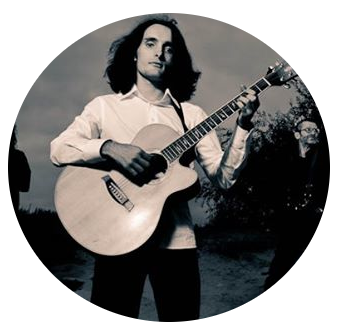
\includegraphics[width=.5\textwidth]{imgs/vlad.png}
}

\only<2> {
    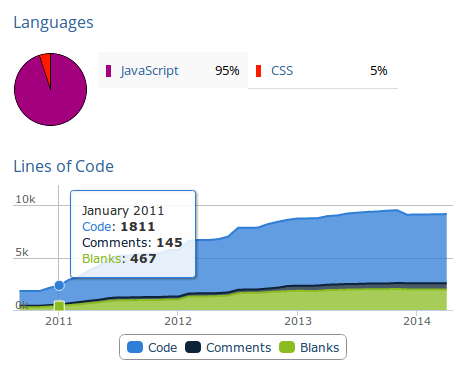
\includegraphics[width=.7\textwidth]{imgs/leaflet-code.png}\\
    \url{http://www.ohloh.net/p/Leaflet/}
}

\only<3> {
    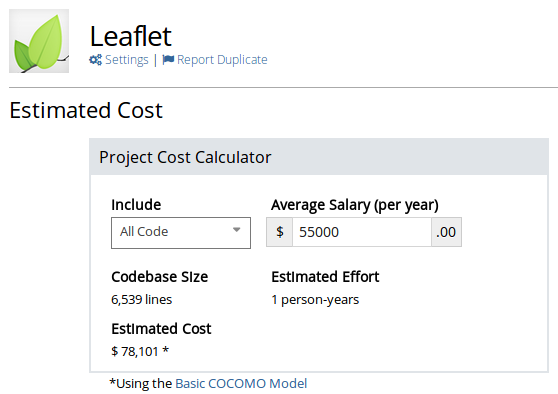
\includegraphics[width=.7\textwidth]{imgs/leaflet-costs.png}\\
    \url{http://www.ohloh.net/p/Leaflet/}
}

\only<4-5> {
    \begin{itemize}
        \item 2010
        \item Méně je někdy více
        \item Omezená práce s projekcemi
        \item Generalizace na straně klienta
        \item Canvas pro vykreslování
    \end{itemize}
}

\only<6>{
    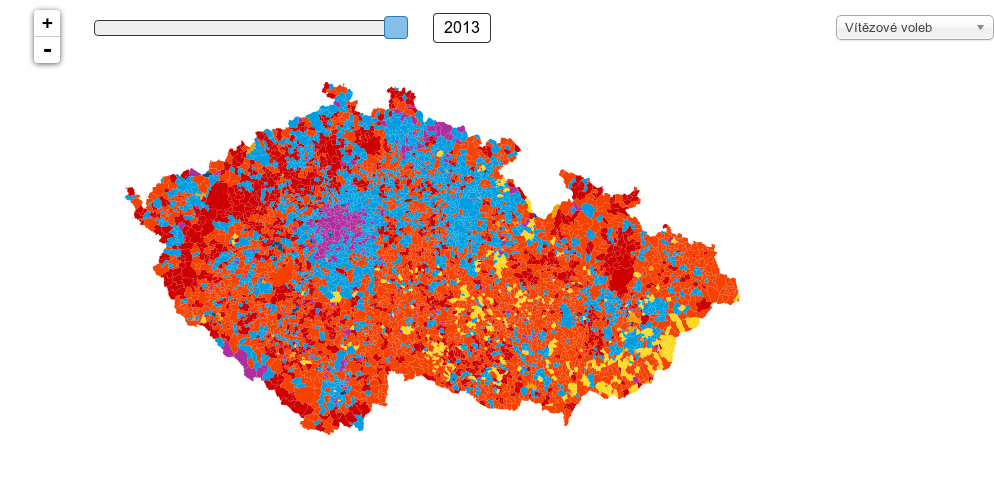
\includegraphics[width=.7\textwidth]{imgs/volby-ihned.png}\\
    \url{http://data.blog.ihned.cz/c1-61086960-jak-se-zmenila-politicka-mapa-republiky-vysledky-snemovnich-voleb-v-kazde-obci-od-roku-1996-do-vcerejska}
}

\only<7> {
    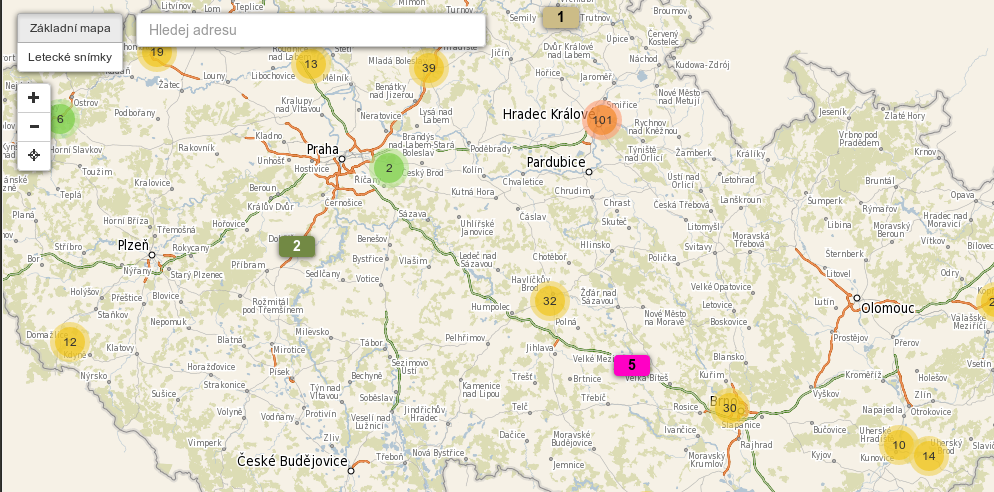
\includegraphics[width=.7\textwidth]{imgs/volby-tmapy.png}\\
    \url{http://volby.tmapy.cz/}
}

\only<8>{
    \includegraphics[width=.7\textwidth]{imgs/github-leaflet.png}\\
    \url{https://github.com/jachym/datamining/blob/master/data/metro.geojson}
}

\note<1>{
    Ten člověk se
    jmenoval Vladimir Agafonkin, je z Ukrajiny, i když dnes se pohybuje spíše ve
    Spojených státech a vytvořil knihovu Leaflet.
}

\note<2>{
    Leaflet je nepoměrně menší projekt. Obsahuje cca 6000 řádků kódu
}

\note<3>{
    náklady jsou odhadnuty na \$78 000, tedy přibližně 20x menší, než u OpenLayers.
}

\note<4>{
    Projekt začal okolo roku 2010 a nabral úžasnou dynamiku - do této chvíle měl 180 přispěvatelů
    (což je dokonce o 66 více, než OpenLayers).  Získal si ohromnou popularitu i
    přesto - nebo právě proto - že obsahuje oproti OpenLayers asi 1/10 funkcí. Např.
    podpora projekcí a souř. systémů je žalostná ve srovnání s OpenLayers, kde
    můžete na klientské straně transformovat vektorová data mezi souř. systémy,
    Leaflet umí v podstatě jenom Googlí Mercator projekci, o S-JTSK si můžete nechat
    zdát. Vladimir je původem matematik a baví ho vymýšlet různé zlepšováky a
    algoritmy.
}

\note<5>{
    Leaflet zavedl celou řadu generalizujících algoritmů vektorových dat,
    které umožňují zobrazovat velké objemy vektorových dat přímo na klientovi.
    Začínáme se tady bavit o v postatě GISových technikách, jak jsou prostorové
    indexy, generalizace, topologické operace a podobně. Stejně jako na desktopu,
    tak i u vektorů platí, že nejnáročnější operace je vykreslení vektorů. Vyplatí
    se data 3x prohnat nějakým algoritmem, který sníží počet vykreslovaných objektů
    na minimum. To Vladimir pochopil a zavedl a slaví s tím úspěch. OpenLayers 2 si
    tyto věci nemohli dovolit kvůli zpětné kompatibilitě. Vladimir vesele s každou
    další verzí Leafletu odstraňuje funkce, místo aby je přidával a dělá tak Leaflet
    ještě rychlejším. OpenLayers stále funkce přidává. Leaflet je tedy malá
    knihovna, která dělá jednu věc - zobrazování dat - a dělá to fakt dobře.
}

\note<6->{
    OpenLayers je na druhé straně vyspělé prostředí GIS, které vám umožní provádět
    na webovém prohlížeči plnohodnotné GIS operace. Leaflet si našel cestu zejména
    do médií. Používají ho Hospodářské noviny (resp. server. IHned)\mynext\\
    ~\\
    a  nedávno jste si mohli všimnout aplikace Volby od firmy T-Mapy.\mynext\\
    ~\\
    Možná jste slyšeli, že i server pro hosting zdrojových kódů GitHub umí,
    pokud do něj uploadnete soubor ve formátu Geo- nebo TopoJSON, jej přímo
    zobrazit
}

\end{center}
\end{frame} % leaflet

%%%%%%%%%%%%%%%%%%%%%%%%%%%%%%%%%%%%%%%%%%%%%%%%%%%%%%%%%%%%%%%%%%%%%%%%%%%%%%%%%%%%%
\begin{frame} % openlayers 3
\begin{center}
\begin{flushright}
    \includegraphics[width=0.08\textwidth]{imgs/ol3.png}
\end{flushright}

\only<1-4>{
    \begin{itemize}
        \item 2D a 3D
        \item Canvas vs \st{DOM}
        \item Generalizace a kartografie na straně klienta
        \item Closure library $n\times{}MB \rightarrow n\times{}KB$
    \end{itemize}
}

\only<5>{
    \includegraphics[width=0.6\textwidth]{imgs/ol-hangout.png}
}

\only<6>{
    \includegraphics[width=0.6\textwidth]{imgs/swisstopo.png}\\
    \url{http://map.geo.admin.ch}
}

\only<7>{
    \includegraphics[width=0.6\textwidth]{imgs/geosense.png}\\
    ~
}


\note<1>{
    Nicméně doba se nezastavila. V roce 2012 byly započaty práce na zcela nové
    knihovně OpenLayers 3. Vývojový team v čele s firmami Boundless a Camp2Camp
    hodil za hlavu zpětnou kompatibilitu a navrhnul mapovou knihovnu pro toto
    desetiletí. OpenLayers 3 jsou momentálně ve fázi BETA a snad během letošního
    jara by měla být uvolněna první verze, která by měla podporovat zhruba to, co
    umí OpenLayers 2. Při přechodu ze starých OpenLayers na nové máte pocit, že věci
    jsou více komplikované, ale při hlubším seznámení zjistíte, že to celé dává
    smysl.
}
\note<2>{
    OpenLayers 3 zavádějí podporu pro 2D i 3D zobrazení přímo v mapě. Data
    jsou vykreslována pomocí Canvasu a WebGL - to nám umožňuje pracovat s datasety
    to deseti tisích prvcích. Dříve se používala technika DOM - document object
    model, která je absolutně neefektivní. Pokud jste někdy dělali jednoduché webové
    stránky, můžete si představit, že každý vektorový objekt je samostatný element,
    který se musí na stránce vykreslit. To je neuvěřitelně neefektivní. Moderní
    prohlížeče podporují tzv. Canvas - jakési rastrové plátno, do kterého můžete
    objekty vykreslit a vše je zobrazeno najednou jako obrázek. To používá částečně
    i Leaflet, ale OpenLayers 3 to používají především. Také OpenLayers 3 zavedli
    generalizační algoritmy, takže se vykresluje jenom to, co vykreslovat smysl má. 
}
\note<3>{
    OpenLayers 3 jsou napsány za pomocí Google Closure library. Výsledkem je, že
    většina neduhů jazyka JavaScript se do jisté míry eliminuje. Nevím, jestli
    seledujete dění okolo jazyka JavaScript v poslední době, ale opravdu prošel
    dynamickým vývojem. Od pomocného jazyka sloužícího k obarvení nadpisu na
    červeno, se zněj stala plnohodnotná programovací platforma s možností typové
    kontroly, unit testy, kompilací kódu a tak dále. JavaScript dávno není jazykem
    webových prohlížečů, ale je spouštěn na serverech, vznikají vazby do dalších
    knihoven. Osobně se domnívám, že JavaScript je budoucí Geo- programovací jazyk,
    podobně jako jím je dnes Python.
}
\note<4>{
    Díky Closure můžeme tzv. vybuildit - sestavit a
    zkomprimovat - mapovou aplikaci na míru, obsahující pouze potřebné komponenty.
    OpenLayers 3 už jsou nasazovány v produkčním prostředí, přesto že jsou sotva ve
    fázi beta a podstatné části knihovny se stále mění pod rukama vývojářů. Jak je
    to možné?
}
\note<5>{
    Je to Open Source software, každý může sledovat vývoj on-line, můžete
    se zúčastnit týdenních porad vývojového teamu přes Google Hangout. Na dotaz do
    mailing listu dostanete relevantní odpověď do půl hodiny. Můžete tedy velice
    dobře ohodnotit, do jakého rizika a nestability jdete a nikdo vám neplánovaně
    nepodtrhne nohy. Každá změna je transparentní, dokumentovaná (pořád se bavíme o
    dynamicky vyvíjeném, software), a je na vás, kdy ji začleníte do svého projektu.
    Máte možnost ale vždy vědět, na čem jste. Tím, že je to zatím opravdu Beta, se v
    české republice zatím moc dobrodruhů nenašlo, kteří by OL3 nasadily.
}
\note<6>{
    OL3 už jsou použity na mapovém portále Švýcarska
}

\note<7>{
    Ve firmě
    Geosense pracujeme na nové prohlížečce geodat, která je kompletně postavená nad
    Closure a OL3. Jak ale praví klasik: chození po vodě a psaní software proti
    standardům je jednoduché, pokud je obojí zamrzlé. OL3 jsou zatím pohyblivý cíl.
}

\end{center}
\end{frame} % openlayers 3

%%%%%%%%%%%%%%%%%%%%%%%%%%%%%%%%%%%%%%%%%%%%%%%%%%%%%%%%%%%%%%%%%%%%%%%%%%%%%%%%%%%%%%
\begin{frame} % open source javascript mapping frameworks
\begin{center}
\includegraphics[width=0.2\textwidth]{imgs/ol.png}\vspace{0.1\textwidth}
\includegraphics[width=0.2\textwidth]{imgs/leaflet.png}\vspace{0.1\textwidth}
\includegraphics[width=0.2\textwidth]{imgs/ol3.png}

\note<1>{
    Podíváme-li se na tyto tři knihovny vedle sebe, pak generačně vzato jsou OL2
    nejníže, Leaflet někde mezi OL2 a OL3 a OpenLayer 3 považuji v tuto chvíli za
    nejvyšší vývojový stupeň. Chcete-li zobrazit mapičku, pravděpodobně použijete
    Leaflet. Chcete-li víc, asi sáhnete po některé z OpenLayers. Pokud nepotřebujete
    zrovna nejmodernější techniky, OL2 jsou stále dobrá, stabilní a prověřená
    platforma.
}
\note<2>{
    Díky možnostem dneších prohlížečů se zcela změnil problém vykeslování dat na
    prohlížeči. Už jsem zmínil, že vykreslit deseti tisíce prvků není problém.
    Problémem je přenos těchto dat ze strany serveru na klienta. Rastrová data
    bývají používána pouze jako podkladové dlaždicované mapy. Veškerá vektorová data
    jsou trasnportována na klienta a tam se odehrává vlastní kartografické
    stylování. To poskytuje obrovské možnosti analýzám a vizualizacím přímo ve
    webovém prohlížeči. Jak ale data přenést?
}
\note<3>{
    Asi chápete, že ESRI Shapefile není nejvhodnější formát. I když existují webové
    zobrazovačky Shapefilů, daleko jednodušší je použít nějaký textový formát typu
    XML nebo JSON. Od XML se v poslední době odkláníme pro jeho ukecanost a
    systémovou nenažřanost - smím-li to tak říct. Moderní formáty založené na JSON
    jsou dobře čitelné a přitom řádově menší. V oblasti GIS používáme samozřejmě
    rošíření GeoJSON. Nejedná se o de-jure standard, ale otevřený a uznávaný
    de-facto standard. Prohlížeče mají menší problém s jejich parserováním, nedojde
    tak snadno k zahlcení prohlížeče. Jak ale "protlačit" desítky tisíc polygonů -
    což odpovídá desítkám megabajtů dat - ze strany serveru na klienta, když máte
    např. mobilní připojení tak, aby uživatel nebyl nucen si jít uvařit kafe, než se
    "to" načte?
}
\end{center}
\end{frame} % open source javascript mapping frameworks
    
%%%%%%%%%%%%%%%%%%%%%%%%%%%%%%%%%%%%%%%%%%%%%%%%%%%%%%%%%%%%%%%%%%%%%%%%%%%%%%%%%%%%%%
\begin{frame} % formats
\begin{center}

\only<1-3>{
    \begin{itemize}
        \item<1->GML $\rightarrow$ GeoJSON
        \item<2->GeoJSON 80MB $\rightarrow$ GZIP $\rightarrow$ 6.7MB
        \item<3->GeoJSON 80MB  $\rightarrow$ TopoJSON $\rightarrow$ 3.3MB
        $\rightarrow$ GZIP $\rightarrow$ 473KB
    \end{itemize}
}
\only<4>{
    \includegraphics[width=0.6\textwidth]{imgs/tilestash.jpg}\\
    \url{http://tilestache.org/}
}

\note<1-2>{
    Základem je komprese komunikace mezi serverem a klientem. Webový server Apache
    např. umí data transparentně zipovat.\mynext\\
    ~\\
    Webový prohlížeč je na druhé straně sám
    rozbalí a předá aplikaci. Tím můžete ušetřit desítky procet datového toku a je
    to pouze otázka jednořádkové konfigurace serveru. ~\\
    ~\\
    Další možností je data kompriovat ještě agresivněji, např. převodem na binární
    podobu. Trochu tím více zatížíte server a klienta, na druhou stranu data tečou
    rychleji. To dokáže např. formát MessagePage, který umožní JSON formáty převézt
    na binární a zpět.
}
\note<3>{
    Další možností je oříznout data jako taková, např. tím, že na klienta půjdou v
    topologicky čisté podobě. V případě polygonů opět můžete ušetřit desítky procent
    z objemu dat jenom tím, že "rozpustíte" dvojité hranice mezi sousedními
    polygony. Opět to klade určitou náročnost na klienta při zpracování, ale z
    pohledu uživatele se "něco děje". To umí např. formát TopoJSON.\mynext\\
    ~\\
    Při dalším zasipování už to začíná být zajímavé
}

\note<4>{
    Poslední mě známou technikou je data rozkouskovat a posílat je na klienta
    postupně - po dlaždicích. Hovoříme o dlaždicovaných vektorech, jejichž asi
    nejvyšší evoluční stupeň je dlaždicovaný TopoJSON. Před uživatelem se tak mapa
    vykresluje postupně, můžeme vektory předcachovat na straně serveru a o to
    rychleji je pak vybavovat ke klientovi. Objem dat se tím nezmění, ale jejich
    přenos se v čas rozloží. 
}
\end{center}
\end{frame}

%%%%%%%%%%%%%%%%%%%%%%%%%%%%%%%%%%%%%%%%%%%%%%%%%%%%%%%%%%%%%%%%%%%%%%%%%%%%%%%%%%%%%%
\begin{frame} % formats
\begin{center}
\only<1>{\alert{de-\textbf{facto} $\times$ de-\textbf{jure}}}
\only<2>{
    \includegraphics[width=0.5\textwidth]{imgs/no-ogc.png}
}
\only<3>{
    \includegraphics[width=0.5\textwidth]{imgs/Mil-aero2.png}
}
\only<4>{
    \includegraphics[width=0.5\textwidth]{imgs/IMG_20140325_101329.jpg}
}
\note<1-3>{
    Už jsem zmínil, že ani GeoJSON, ani TopoJSON nejsou formálně vzato standardní
    formáty. O jejich vývoj (naposledy v GeoJSONu je přidávána podpora pro časovou
    složku) se stará komunita, které může být součástí každý.\mynext~\\
    ~\\
    Konsorcium OGC trochu
    zaspalo a sám jsem zvědavý, jak se situace okolo GeoJSON a TopoJSON bude
    vyvíjet.\mynext\\
    ~\\
    Důležité ale je, že jsou to standardy otevřené, každý je může studovat,
    měnit, dále distrubuovat a implemenvat do svého software.\mynext~\\
}
\note<4>{
    Naposledy se takto
    sešly projekty MapServer, OpenLayers, QGIS, PostGIS a další tento rok ve Vídni a
    diskutovali spolu vývoj právě dlaždicovaného vektorového topologického formátu.
    Rád bych řekl, že je všechno růžově krásné a spolupracující, ale není. Svět Open
    Source je do určité míry světem chaosu a pravdou je, že takový dlaždicovaný,
    kompriovaný, topologický a nově i otevřený formát už existuje. Jeho nevýhoda je,
    že jej vytvořila jedna firma pro svou potřebu, za zavřenými dveřmi a i když jej
    teď nabízí komunitě, začátek nebyl šťastný. Google kdysi se svým formátem KML
    uspěl (kde je dneska KML?), snad se to podaří i MapBoxu.
}
\end{center}
\end{frame}

%%%%%%%%%%%%%%%%%%%%%%%%%%%%%%%%%%%%%%%%%%%%%%%%%%%%%%%%%%%%%%%%%%%%%%%%%%%%%%%%%%%%%%
\begin{frame} % mapbox
\begin{center}

\only<1>{
    \includegraphics[width=1\textwidth]{imgs/mapbox.png}\\
    \url{http://mapbox.com}
}

\only<2>{
    \url{https://www.mapbox.com/blog/mapbox-js-with-leaflet/}
    \begin{itemize}
        \item Straightforward API
        \item Stable
        \item Plugins
        \item Tested and Supported
    \end{itemize}
}

\only<3>{
    \includegraphics[width=1\textwidth]{imgs/mapbox-satelite.png}
}

\note<1-2> {
    MapBox je americká firma, která se bez nadsázky snaží uspět proti Google Maps na
    globálním trhu. Nabízí pokladové mapy a (zatím) družicové snímky za rozumných
    finančích podmínek. Řada jejich produktů je Open Source, např. nástroj pro
    správu dalždicových cashí TileMill.\mynext\\
    ~\\
    Mezi jejich zaměstnance patří nově i
    Vladimir Agafonkin a i když jejich API podporuje i další knihovn a standardní
    rozhraní, Leaflet je vzat jako jejich výchozí knihovna.
}

\note<3>{
    Už jsem říkal, že pokladové letecké snímky jsou vlastně snímky satelitními.
    Topografický poklad používá kompletně projekt OpenStreetMap. Většinu dat si ale
    můžete ostylovat na klientovi. MapBox k tomuto účelu vyvinuly právě úsporný
    formát pro přenos dat na klienta.
}
\end{center}
\end{frame} % mapbox

%%%%%%%%%%%%%%%%%%%%%%%%%%%%%%%%%%%%%%%%%%%%%%%%%%%%%%%%%%%%%%%%%%%%%%%%%%%%%%%%%%%%%%
\begin{frame} % d3js
\begin{center}
\only<2>{
    \includegraphics[width=0.5\textwidth]{imgs/d3.png}\\
    \url{http://d3js.org}
}
\only<3>{
    \includegraphics[width=1\textwidth]{imgs/d3js-about.png}\\
}

\only<4>{
    \includegraphics[width=1\textwidth]{imgs/d3js-map.png}\\
}
\only<5>{
    \includegraphics[width=1\textwidth]{imgs/d3js-hn.png}\\
    \url{http://datablog.ihned.cz}
}

\only<6>{
\includegraphics[width=0.5\textwidth]{imgs/osm3d.jpg}\\
    \url{http://osmbuildings.org}
}

\note<1>{
    To bychom měli základní přehled OpenSource JavaScriptových frameworků. Co
    dodat?\mynext\\
    ~\\
    Dodám D3.js
}
\note<2>{
    O D3.js toho moc nevím, protože ve své denní práci používám knihovny, které
    mi umožňují stavět cokoliv od aplikací, přes mapové portály až po něco, čemu
    se vznešeně říká Web GIS. D3.js je jiná. 
}
\note<3>{
    D3.js je knihovna v jazyce javascript, sloužící k manipulaci dokumentů,
    založených na datech. Používá standardní HTML, SVG a CSS techniky a nad nim
    staví celkem slušně schopnou vizualizační platformu.
}
\note<4>{
    Obsahuje také podporu pro kartografické vizualizace a já se osobně domnívám,
    že je na velice slušné úrovni. Kde byste mohli mít problém, je množství
    objektů, které půjde rozumně zobrazit, což je dáno limity použitých technik,
    hlavně DOM.
}
\note<5>{
    Nicméně na ilustrační živé mapy je to perfektní technologie. U nás ji
    používají opět např. na datablogu HN
}

\note<6>{
    Je toho samozřejmě mnohem více. Okolo těchto knihoven existuje ekosystém
    nadstaveb, zásuvných modulů a odvozených projektů, např. GeoExt nebo
    HSLayers nebo OSMBuildings abych jmenoval alespoň některé.
}
\end{center}
\end{frame} % d3js


%%%%%%%%%%%%%%%%%%%%%%%%%%%%%%%%%%%%%%%%%%%%%%%%%%%%%%%%%%%%%%%%%%%%%%%%%%%%%%%%%%%%%%
\begin{frame} % závar
\begin{center}

\only<2>{
    \includegraphics[width=0.7\textwidth]{imgs/os-or.png}
}

\only<3>{
    \includegraphics[width=0.7\textwidth]{imgs/os-and.png}
}

\only<4>{
    \includegraphics[width=0.7\textwidth]{imgs/no-marketing.png}
}

\note<1-3>{
    Rád bych na závěr přidal pár rad, jakým způsobem nejlépe zvolit to správné prostředí. Dobrá
    správa je, že ať nasadíte na serveru cokoliv, můžete vyměnit front-end a
    obráceně, výměna front-endové knihovny nezakládá důvod pro změnu back-endu -
    pokud tedy používáte oteřevné, vzájemě interoperabilní knihovny.\mynext\\
    ~\\
    Otázka nestojí, jestli zvolíte ten nebo ten softwarový stack, ale\mynext\\
    ~\\
    Můžete si vybrat mezi vzájemně kompatibilními platformami -- sejdou-li se na
    otevřených standardech
}

\note<4>{
    Už jsem říkal, že Open Source nemá marketingové oddělení. Nikdo vám neukáže
    světélkující prezentaci s úžasnými funkcemi, žádný obchodník za vás to
    rozhodnutí neudělá. Nemusíte podepisovat žádnou smlouvu, musíte se "jenom"
    rozhodnout. Takže jak?
}
\end{center}
\end{frame}

%%%%%%%%%%%%%%%%%%%%%%%%%%%%%%%%%%%%%%%%%%%%%%%%%%%%%%%%%%%%%%%%%%%%%%%%%%%%%%%%%%%%%%
\begin{frame} % závar
\begin{center}
\only<1>{
    \begin{itemize}
        \item Historie
        \item Komunita
        \item Zdrojový kód
    \end{itemize}
}

\only<2>{
    \includegraphics[width=.7\textwidth]{imgs/ol-ohloh-code.png}\\
    \url{http://ohloh.org/p/openlayers}
}

\only<3>{
    \includegraphics[width=1\textwidth]{imgs/ol3-github.png}\\
    \url{http://github.com/openlayers/ol3}
}

\only<4>{
    \includegraphics[width=.5\textwidth]{imgs/OSGeo_logo_750_317.png}\\
    \url{http://osgeo.org}
}

\only<5>{
    \includegraphics[width=.5\textwidth]{imgs/freegeocz.png}\\
    \url{http://mailman.fsv.cvut.cz/mailman/listinfo/freegeocz}
}

\only<6>{
    \includegraphics[width=.5\textwidth]{imgs/nobridge.png}
}

\only<8>{
    \includegraphics[width=.5\textwidth]{imgs/community.jpg}
}

\note<1>{
    Evaluačními kritérii pro výběr Open Source projekt je pro mě historie zdrojového
    kódu. Pokud se projekt dlouho nevyvíjí, může to znamenat, že je vše hotovo.
    Častěji to ale znamená, že je mrtvý. Dalším kritériem je velikost a stabilita
    komunity. Existuje mailing list? Je na něm provoz? Jak rychle dostatete odpověď?
    Důležitá je dokumentace - lze ji použít? Dává návod? Pokud to umím, podívám se
    na zdrojový kód a na to, jaký na mě udělá dojem. To jsem ale schopen udělat
    pouze u několika projektů a popravdě - raději to nedělám, pokud nemusím.
}

\note<2-3>{
    Určitým vodíkem vám může být aktivita, kterou jednoduše uvidíte např. na serveru
    Ohloh\mynext\\
    ~\\
    nebo Github.
}
\note<4>{
    Dále jsou zde různé organizace, zejména Open Souce
    Geospatial Foundation - OSGeo.org. OSGeo certifikuje Open Source projekty,
    hodnotí velikost a aktivitu komunity, kvalitu zdrojového kódu, rozhodovací
    procesy v komunitě atd atd. Je-li nějaký projekt OSGeo-projekt, znamená to, že
    je stabilní a kvalitní. Na okraj: OpenLayers jsou OSGeo projekt, Leaflet není,
    což není z důvodu jeho nekvality, ale protože Vladimir Agafonkin prostě nechce.
    Z tohoto pohledu je Leaflet one-man-show (i když má 180 přispěvatelů), zatím co
    OSGeo-projekty řídí project steering committee.
}

\note<5>{
    Pořád nevíte? Zeptejte se na mailing listu. V Česku existuje freegeocz mailing
    list, na kterém je většina nás uživatelů i vývojářů OSS a rádi vám poradíme.
    Máte se kde zeptat, ale musíte s zeptat.
}

\note<6>{
    Může se stát, že na váš úkol neexistuje Open Source odpověď. V tom případě máte
    dvě možnosti: zvažte, jestli je ve vašich silách jakkoliv přispět do
    existujícího projektu nebo vytvořit nový - je to tak snadné. Nebo jděte do
    proprietárního software. Buďte si ale vždy vědomi, proč to děláte a co tím
    ztrácíte.
}

\note<7-8>{
    Máte chuť jít do Open Source? Především, začněte na malém projektu, zkuste jak
    to funguje. Dejte vývojářům a sami sobě čas na učení a experimentování. Na jednu
    stranu jste v tom sami - neexistuje marketingové oddělení.\mynext\\
    ~\\
    Ale na druhou stranu
    stojí za vámi komunita o kterou se můžete opřít. A jsou zde i firmy či
    jednotlivci, nabízející profesionální konzultační šlužby a podporu pro různé
    projekty, i v České republice.
}

\end{center}
\end{frame}

%%%%%%%%%%%%%%%%%%%%%%%%%%%%%%%%%%%%%%%%%%%%%%%%%%%%%%%%%%%%%%%%%%%%%%%%%%%%%%%%%%%%%%
\begin{frame} % závar
\begin{center}
twitter: @jachymc\\
e-mail: jachym@les-ejk.cz\\
\url{http://github.com/jachym}\\
\includegraphics[width=.3\textwidth]{imgs/licence.png}
\end{center}
\end{frame}
